\chapter{Sistemas Vestíveis} 
\label{cap:wearablw_systems}

Sistemas Vestíveis podem ser definidos como dispositivos eletrônicos móveis que podem ser discretamente embutidos nos trajes do usuário, como parte da roupa ou um acessório. Diferente dos sistemas móveis convencionais, eles podem funcionar sem ou com muito pouca interferência nas atividades do usuário \citep{lukowicz2004wearable}. 

Hoje, muitos destes dispositivos vestíveis vem com uma gama de sensores embutidos que são utilizados na detecção de quedas. O tipo de sensor mais comum utilizado em \ac{FDS} é o acelerômetro, com alguns desses sistemas também utilizando o giroscópio como um sensor auxiliar. De acordo com a revisão sistemática feito por \cite{igual2013challenges}, 186 dos 197 sistemas analisados utilizam o acelerômetro como sensor principal na detecção de quedas. A utilização desde sensores em \ac{FDS} se deve muito pela popularização e o barateamento dos mesmos, além da utilização desses sensores embarcados em smartphones e smartwatches.


As seções desse capítulo são organizadas da seguinte maneira: A seção \ref{sec:sensors} descreve os principais tipos de sensores utilizados em \ac{FDS}; A \ref{sec:sensor_position} fala sobre o posicionamento de sensores, fazendo uma correlação entre o posiciomanento dos sensores e a accurâcia dos sistemas estudados; A seção \ref{sec: FDS_algorithm} fala sobre os diferentes tipos de algoritmos de detecção de quedas mostrando suas vantagens e desvantagens; Por fim, a seção \ref{sec:FDS_examples} irá mostrar exemplos de aplicações que realizam a detecção de quedas atravês de tecnologias vestíveis. 



\section{Sensores}
\label{sec:sensors}
A escolha e o bom funcionamento de sensores são uma parte essencial no bom funcionamento de sistemas de detecção de quedas. De forma geral, sensores são dispositivos que convertem fenômenos físicos em sinais elétricos. Sendo assim , eles representam a camada de comunicação entre o mundo físico e o mundo digital. 

Os dois tipo principais de sensores utilizados em sistemas de detecção de queda são o acelerômetro e o giroscópio. Eles fazem parte de um grupo chamado de \ac{MEMS}. Estes sensores são geralmente feitos de chips de silício utilizando as mesmas técnicas usadas na confecção de chips de computadores pessoais. Para que um sensor possa ser classificado como \ac{MEMS} alguma parte do seu design precisa vibrar ou se mover de alguma forma \citep{milette2012professional}. 

De forma geral tanto o acelerômetro quanto o giróscopio utilizam 3 eixos para expressar seus valores. O sistema de coordenadas utilizado é relativo a cada dispositivo. Na figura \ref{fig:axis_device} temos  exemplo do sistemas de coordenadas utilizado pelo sistema operacional Android\footnote{https://www.android.com/}. Neste sistema o ponto de origem é o centro da tela do dispositivo, quando segurado na posição vertical \citep{sensorAndroidDocs}. 

\begin{figure}[ht]
	\centering
	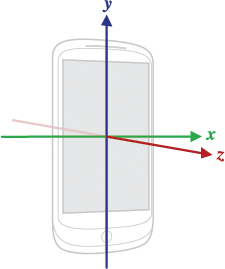
\includegraphics[scale=0.6]{imagens/axis_device.png}
	\caption{Sistema de coordenadas utilizado pelo sistema operacional Android \citep{sensorAndroidDocs}.}
	\label{fig:axis_device}
\end{figure} 

\subsection{Acelerômetro}
\label{subsec:accelerometer}
Fisicamente, o acelerômetro é um dispositivo composto de uma pequena massa  anexado a pequenas molas que são utilizadas para medir a aceleração aplicada sobre um dispositivo, incluindo a força da gravidade. A aceleração é medida analisando o quanto a massa se distancia do seu ponto de equilíbrio. 

\begin{figure}[ht]
	\centering
	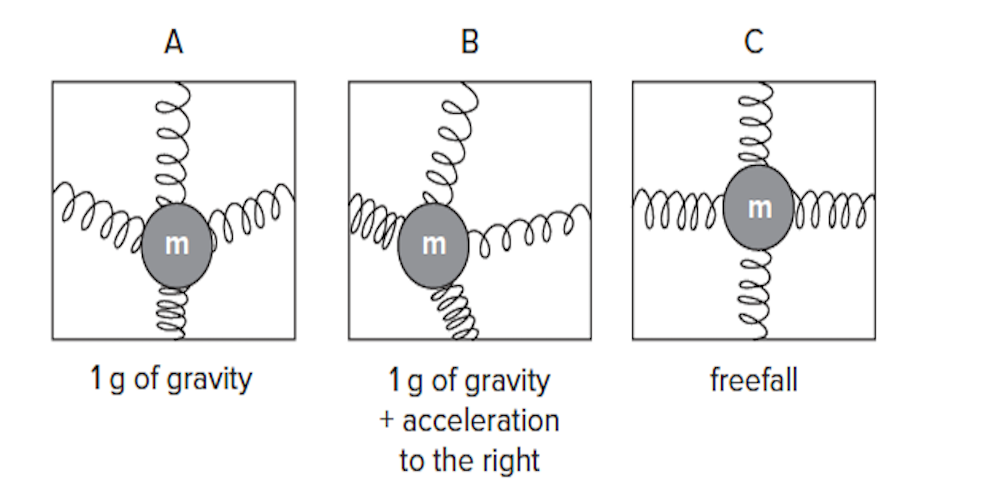
\includegraphics[scale=0.6]{imagens/MEMS_device.jpg}
	\caption{Força sendo aplicando sobre uma massa presa a molas \citep{milette2012professional}.}
	\label{fig:acelerometro}
\end{figure} 

	
Na figura \ref{fig:acelerometro} em A é possível ver um aparelho parado em uma mesa, sobre ele só irá agir a força de gravidade 1G de aproximadamente $9.8 m/s^{2}$. Em  B, o aparelho foi jogado para a direita, então irá agir sobre ele, além da força da gravidade, uma aceleração no sentido para onde o aparelho se movimentou. Já em C, vemos um aparelho em queda livre com aceleração no sentido oposto a força da gravidade, o que faz com a massa fique localizada em seu ponto de equilibrio, e a força resultante  seja de $0G$ \citep{milette2012professional}.


\subsection{Giroscópio}
	
	O giroscópio, similarmente aos acelerômetros, são pequenas massas em pequenas molas, só que em vez de medir a aceleração, são utilizados para medir um tipo de força chamada de Força de Coriolis. A Força de Coriolis é a tendência que um objeto livre possui de sair do curso quando visto de um ponto de referência em rotação \citep{milette2012professional}. Por exemplo, se sentarmos em um carrosel e rolarmos a bola pra longe, a bola irá parece desviar em uma linha reta, como se existisse uma força agindo sobre ela. Esta força é chamada de Força de Coriolis.
	
	Apesar de possuir uma estrutura física semelhante, o aceletrometro e o giroscópio se diferem em seu funcionamento. Em vez de esperar a força da gravidade agir sobre a massa, o giroscópio funciona vibrando está massa sobre o eixo definido. Quando o giroscópio é rotacionado, a Força de Coriolis faz com que a massa comece a ser mover em um eixo dirente no qual ele estava vibrando anteriomente.  \cite{milette2012professional}.
	
	Como a força de Coriolis age somente quando o dispositivo está em rotação, o giroscópio só é capaz de calcular a velocidade angular, ou seja, a velocidade com que o aparelho está sendo rotacionado. 
	
	A orientação da dispositivo irá definir quando o valor da rotação será positivo ou negativo. Nos dispositivos Android, a velocidade Angular é medida em radianos por segundo ($rad/s$) e é positiva em rotações no sentido anti-horário \citep{GyroscopeAndroidDocs}. 
	
\section{Posicionamento de Sensores}
\label{sec:sensor_position}

O posicionamento dos sensores afeta diretamente a performance dos \ac{FDS}, dependendo da posição onde colocamos os sensores, o sistema pode indicar uma maior ou menor quantidade de falhas. 

Não existe um consenso sobre a posição otimizada dos sensores para que se possa realizar a detecção de quedas. De acordo com \cite{abbate2011recognition}, a cintura seria o local ideal para o posicionamento, já que estaria mais perto do centro de gravidade do corpo humano. Entretanto em \cite{kangas2007determination}, já foi sugerido que a cabeça seria o melhor lugar para posicionar os sensores. Outras soluções, como em \cite{gjoreski2011accelerometer}, já propõem o uso de mais de um sensor, colocando-os em diferentes partes do corpo com o objetivo de aumentar ainda mais a precisão dos \ac{FDS}.


De acordo com X, o pulso não é o local recomendado para o posicionamento de sensores em sistemas de detecção de quedas. Isso se deve  a constante movimentação dos braços, que podem gerar um número grande de falso-positivos. Entretanto, alguns sistemas tem conseguido resultados satisfatórios com \ac{FDS} localizados no pulso. O sistema proposto por \cite{hsieh2014wrist}, foi capaz detectar quedas em 151 das 160 quedas simuladas e obteve uma especificidade (capacidade de não reconhecer eventos de quedas, como tal) de 95\%.

Além da acurrácia do sistema, outras questões precisam ser levadas em consideração quando pensamos no posicionamento dos sensores. Uma delas é a danificação dos sensores na occorrência de uma queda. Caso o sistema pare de funcionar, um possível alerta de emergência poderá não ser enviado e o idoso poderá está correndo grande perigo. 

Outra questão é a usabilidade, o uso de muitos sensores, apesar de poder elevar a precisão do sistema, poderá levar a um disconforto do usuário, que pode fazer até com que o mesmo desista de usá-lo. 


\section{Algoritmos de Detecção de Queda}
\label{sec: FDS_algorithm}
Os algoritmos de detecção de quedas recebem como entrada os dados obtidos através dos sensores e são capazes de determinar se o que ocorreu foi um evento de queda ou somente uma \ac{ADL}. De acordo com \cite{casilari2015analysis}, é possível separar os algoritmos de detecção em dois grandes grupos: Algoritmos de detecção através de métodos de reconhecimento de padrões, algoritmos baseados em limiares. 




\subsection{Reconhecimento de Padrões}
O reconhecimento de padrões é uma área do aprendizado de máquina que foca no reconhecimento de padrões e regularidades de dados \citep{anzai2012pattern}. Diversas técnicas de aprendizado de máquina tem sido empregadas na detecção de quedas, de acordo com a revisão sistemática feita por \cite{casilari2015analysis}, algoritmos como o de \textit{Naïve Bayes}, \textit{Redes Neurais}, e \textit{Árvores de Decisão} tem sido utilizados.


Um exemplo de sistema que utiliza a técnica de reconhecimento de padrões foi proposto por \cite{zhao2012fallalarm}. O seu algoritmo de detecção de quedas analisa dados do acelerômetro através de uma árvore de decisão, assim identificando um evento de queda. 

Este algoritmo é composto de 2 fases, a primeira é o que chamamos em aprendizado de máquina de fase de treinamento. Será realizado a coleta de dado e a  extração das características que são pertinentes, além do treinamento de um modelo de árvore de decisão. Na figura \ref{fig:decision_tree} podemos ver o modelo de árvore de decisão gerado.  Este modelo de árvore de decisão é capaz de reconhecer atividades como andar, correr, estado estático ou um evento de queda através das variáveis \textit{Std\_x}, \textit{Mean\_y} e \textit{Slope} que representam caracteristicas do sistema. 


\begin{figure}[ht]
	\centering
	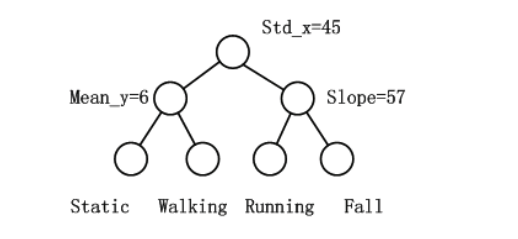
\includegraphics[scale=0.6]{imagens/decision_tree.png}
	\caption{ Modelo de árvore de decisão construida em \cite{zhao2012fallalarm}.}
	\label{fig:decision_tree}
\end{figure} 


Na segunda fase, chamada de fase de testes, o modelo de árvore de decisão é utilizado em uma aplicação no smartphone que será responsável pelo reconhecimento de atividades. Os dados dos sensores são catalogados e transformados nas caracteristicas do sistema, que serviram como dados de entrada da árvore de decisão, que terá como saída o tipo de atividade que foi desempenhada.

Sistemas que utilizam reconhecimento de padrões, normalmente está suscetível a altos custos computacionais, análise massiva de dados, e acesso a grandes bancos de dados ou longos periodos de treinamentos onde o algoritmo de classificação precisa ser parametrizado e adaptado a diferentes grupos de usuários \citep{casilari2015analysis}. Em constraste, existem os algoritmos baseados em limiares que tendem a ser mais simples e similarmente eficientes, desde que encontremos limiares adequados. 

\subsection{Baseado em Limiares}
Algoritmos baseados em limiares utilizados na detecção de quedas comparam os dados dos sensores com um ou mais valores pré-definidos, chamados de limiares. Estes valores podem ser fixos ou adaptados. Quando estes valores são adaptados, eles não mudam dinamicamente enquanto os usuários estão utilizando o sistema. Em vez disso, o usuário irá introduzir dadados sobre o seu perfil fisiológico e o sistema irá informar os limiares adequados \citep{habib2014smartphone}. Um exemplo deste tipo de sistema pode ser visto em \cite{sposaro2009ifall}, o valor limiar mudar de acordo com os parametros providos pelo usuário como altura, peso e nível de atividade. 

De acordo com a revisão sistemática feito por \cite{casilari2015analysis}, muitos sistemas de detecção de queda utilizam o valor de \ac{SMV} do vetor de aceleração como  valor limiar principal em seus algoritmos de detecção. O valor de \ac{SMV} é definido através da equação em \ref{eq:SMV}, onde $X_i$, $Y_i$, $Z_i$, representam, respectivamente, os valores de aceleração dos eixos x, y, z obtidos através do acelerômetro descrito em  \ref{subsec:accelerometer}.

\begin{equation}
SMV = \sqrt{X_i^2 + Y_i^2 + Zi_i^2} 
\label{eq:SMV}
\end{equation}

A escolha dos limiares é um fato determinante para o sucesso deste tipo de algoritmo de detecção de quedas. A escolha dos limiares pode ser feita atravês de experimentos preliminares como em \cite{zhang2013honey}. Em seu trabalho, um grupo de voluntários foi escolhido para realizar diversas \ac{ADL}, como andar, correr subir e descer escadas e também realizar a simulação de quedas. Através dos dados obtidos foi possível descobrir os limiares de \ac{SMV} para um evento de queda.  

De acordo com \cite{cao2012falld}, a performance dos algoritmos aumenta significadamente quando utilizamos valores de limiar dinâmicos. De acordo com sua pesquisa, o número de eventos de queda que não foram caracterizadas como tal, cairam de 53 para 29 quando o peso, sexo idade foram levados em consideração no momento da definição dos limiares.

Outra questão importante quando utilizado este tipo de algoritmo é o número de limiares utilizados. De acordo com \cite{casilari2015analysis}, o uso de um único limiar faz com que o algoritmo emita um número grande de alerta falsos, categorizando \ac{ADL} como eventos de queda, fazendo com que o uso de somente um limiar não seja adequado no desenvolvimento de \ac{FDS}.
\section{Trabalhos Relacionados}
\label{sec:FDS_examples}
d

